\colorlet{mylightgray}{black!30}
\colorlet{mydarkgray}{black!50}

\colorlet{mydarkblue}{blue!50!black}
\colorlet{watercol}{blue!80!cyan!10!white}
\colorlet{darkwatercol}{blue!80!cyan!20!white}

\tikzstyle{plasma}=[very thick, draw=black, top color=mydarkgray, bottom color=mydarkgray]

\tikzstyle{water}=[draw=mydarkblue,top color=watercol!90,bottom color=watercol!90!black,shading angle=5]
\tikzstyle{vertical water}=[water, top color=watercol!90!black!90,bottom color=watercol!90!black!90,middle color=watercol!80,shading angle=90]
\tikzstyle{dark water}=[draw=mydarkblue,top color=darkwatercol,bottom color=darkwatercol!80!black,shading angle=5]


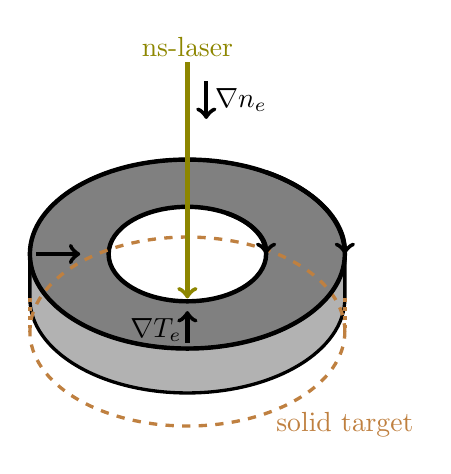
\begin{tikzpicture}[scale=0.4]
  \def\Rx{5.0}      % tank horizontal radius
  \def\Ry{3.0}      % tank vertical radius
  \def\rx{0.5*\Rx} % column horizontal radius
  \def\ry{0.5*\Ry} % column vertical radius
  \def\H{1.5}       % height tank
  \def\h{0.94*\H}   % height water
  \def\l{-0.7*\H}   % height water
  \def\y{0.40*\H}   % vertical position piece
  \def\dy{0.10*\H}  % height piece
  \def\shif{0.6}

  \draw[very thick, fill=mylightgray] (-\Rx,\h) -- (-\Rx,0) arc (180:360:{\Rx} and {\Ry}) -- (\Rx,\h);
  %\draw[very thick, dotted] (-\Rx,0) -- (-\Rx,\l) arc (180:360:{\Rx} and {\Ry}) -- (\Rx,0);
  \draw[fill=mydarkgray, very thick] (0,\h) ellipse ({\Rx} and {\Ry});
  \draw[ultra thick, fill=white] (0,\h) ellipse ({\rx} and {\ry});
  \draw[very thick, dotted, color=brown] (-\Rx,0) -- (-\Rx,\l);
  \draw[very thick, dotted, color=brown] ( \Rx,0) -- ( \Rx,\l);
  \draw[very thick, dashed, color=brown] (0,\l) ellipse ({\Rx} and {\Ry});
  \node[color=brown] at (5.0,-4.0) {solid target};
  \draw[<-, ultra thick] (0+\rx, \h) arc [start angle=0, end angle=60, x radius ={\rx}, y radius={\ry}];
  \draw[ultra thick] (0,\h) ellipse ({\Rx} and {\Ry});
  \draw[<-, ultra thick] (0+\Rx, \h) arc [start angle=0, end angle=60, x radius ={\Rx}, y radius={\Ry}];

  \draw[ultra thick, ->, color=olive] (0, 5*\H) -- (0, 0);
  \node[color=olive] at (0.0, 8.0) {ns-laser};

  \draw[ultra thick, ->] (\shif, 4.6*\H) -- (\shif, 3.8*\H);
  \node at (1.7, 6.3) {$\boldsymbol{\nabla} n_e$};
  \draw[ultra thick, ->] (-4.8, \h) -- (-3.4, \h);
  \draw[ultra thick, ->] (0, -1.4) -- (0, -0.4);
  \node at (-1.0, -1.0) {$\boldsymbol{\nabla} T_e$};


  %%% % COLUMN + PIECE
  %%% \draw[dark water]
  %%%   (-\rx,\y) -- (-\rx,\y-\dy) arc (180:360:{\rx} and {\ry}) -- (\rx,\y);
  %%% \draw[dark water]
  %%%   (0,\y) ellipse ({\rx} and {\ry});
  %%% \draw[dark water,opacity=0.50,draw=none] % column
  %%%   (-\rx,\h) -- (-\rx,\y) arc (180:360:{\rx} and {\ry}) -- (\rx,\h) arc(360:180:{\rx} and {\ry}) -- cycle;
  %%% \draw[blue!20!black,dashed,very thin,opacity=0.50] (-\rx,\y) -- (-\rx,\h) (\rx,\y) -- (\rx,\h);
  %%% \draw[dark water,opacity=0.50] % top column
  %%%   (0,\h) ellipse ({\rx} and {\ry});
  %%% \draw[blue!30!black]
  %%%   (0,\h) ellipse ({\Rx} and {\Ry});
  %%% 
  %%% % CONTAINER
  %%% \draw[thick]
  %%%   (-\Rx,\H) -- (-\Rx,0) arc (180:360:{\Rx} and {\Ry}) -- (\Rx,\H);
  %%% \draw[thick]
  %%%   (0,\H) ellipse ({\Rx} and {\Ry});
  %%% 
  %%% % LABELS
  %%% \node[scale=0.98] at ({-0.45*(\Rx+\rx)},1.04*\h) {$P_\mathrm{atm}$}; %{\contour{watercol}{$P_\mathrm{atm}$}};
  %%% \node at ({-0.40*(\Rx+\rx)},{\y-0.5*\dy}) {$P$};
  %%% \node[above=-2] at (0,\y+\ry) {$A$};
  %%% \draw[<->] (1.2*\Rx,\y) --++ (0,\h-\y) node[midway,fill=white,inner sep=1] {$h$};
  
\end{tikzpicture}

